\documentclass[10pt, reqno, letterpaper, twoside]{amsart}
\usepackage[margin=1in]{geometry}

\usepackage{amssymb, bm, mathtools}
\usepackage[usenames,dvipsnames,svgnames,table]{xcolor}
\usepackage[pdftex, xetex]{graphicx}
\usepackage{enumerate, setspace}
\usepackage{float, colortbl, tabularx, longtable, multirow, subcaption, environ, wrapfig, textcomp, booktabs}
\usepackage{pgf, tikz, framed, url, hyperref}
\usepackage[normalem]{ulem}
% \usetikzlibrary{arrows,positioning,automata,shadows,fit,shapes}
\usepackage[english]{babel}

\usepackage{microtype}
\microtypecontext{spacing=nonfrench}

\usepackage{times}
\usepackage[numbers,sort&compress]{natbib}
\usepackage{xcolor} % Required for colors
\newcommand{\vg}[1]{{\color{blue} vg: #1}} % Shorthand command
\newcommand{\ad}[1]{{\color{red} ad: #1}} % Shorthand command
\newcommand{\es}[1]{{\color{green} es: #1}} % Shorthand command
\newcommand{\pv}[1]{{\color{purple} pv: #1}} % Shorthand command

\usetikzlibrary{arrows.meta, positioning, fit, shapes.misc}
\tikzset{
  box/.style={draw, rounded corners, align=center, inner sep=6pt, minimum width=2.6cm, minimum height=1.0cm},
  sbox/.style={draw, rounded corners, align=center, inner sep=5pt, minimum width=2.4cm, minimum height=0.85cm},
  line/.style={-Latex, thick},
  dashedline/.style={-Latex, thick, dashed},
  note/.style={align=left, font=\small}
}

\title{Circuit Distillation for Math Reasoning: Aligning Computational Mechanisms in Large Language Models}
\author{
Eshan Singhal [esinghal@seas], Audhav Durai [audhav@wharton], \\ Vedant Gaur [vedantg@wharton], Praneel Varshney [pvarsh@seas]
}

\begin{document}

\begin{abstract}
\emph{Circuit Distillation} is a mechanism-level approach to transferring knowledge from a large teacher model to a smaller student by aligning internal computational circuits rather than matching outputs, as in traditional knowledge distillation. We study this approach for arithmetic reasoning in the Llama~3 family through a two-part framework. First, we introduce an ablation-based distillation method that identifies functionally critical MLP layers in both teacher and student models and aligns their internal representations using representational similarity objectives. Second, we propose a complementary neuron-level circuit discovery framework that clusters arithmetic problems into latent classes and learns sparse, functionally distinct neuron masks, providing a fine-grained decomposition of arithmetic computation.

We evaluate circuit distillation on two-digit addition, distilling a Llama-3.2-1B student from a Llama-3-8B teacher. Our method improves student accuracy from 51.6\% to 96.3\%, fully closing the reasoning gap and matching teacher performance. We further observe that minimizing CKA loss between paired computational circuits closely correlates with the emergence of arithmetic capability. The neuron-level circuit discovery results reveal sparse, consistent subcircuits that persist across model scales, suggesting a promising foundation for future fine-grained mechanism-level transfer.
\end{abstract}


\maketitle

\section{Introduction}

Large language models (LLMs) exhibit strong arithmetic and symbolic reasoning abilities when scaled to tens of billions of parameters \citep{dubey2024llama}. However, deploying such models is often infeasible due to computational and memory constraints. Knowledge distillation seeks to transfer capabilities from large teacher models to smaller student models, but conventional approaches primarily focus on matching outputs rather than internal computation. As a result, distilled models may reproduce correct answers while relying on brittle heuristics instead of the teacher’s underlying algorithmic mechanisms \citep{wadhwa2024mysteries}.

Mechanistic interpretability suggests that many reasoning behaviors in transformers are implemented by sparse, functionally specialized subcircuits composed of particular neurons and attention heads \citep{elhage2021mathematical}. This motivates the question: \emph{can we identify such circuits and distill them directly into smaller models?} If so, student models could inherit not just surface-level behavior but the teacher’s internal reasoning process.

In this work, we study \emph{circuit distillation} for arithmetic reasoning through two complementary instantiations. First, we introduce a scalable, ablation-based method that identifies functionally critical layers in both teacher and student models and aligns their internal representations using representational similarity objectives. This approach enables effective mechanism-level transfer and yields strong empirical gains on arithmetic tasks. Second, we propose a neuron-level circuit discovery framework that decomposes arithmetic computation into sparse, latent subcircuits by clustering problems and learning structured neuron masks. While more fine-grained, this framework provides mechanistic insight into how arithmetic reasoning is implemented within transformer models and serves as a foundation for circuit-level distillation.

\subsection{Contributions}

\begin{itemize}
\item We study circuit distillation through two complementary mechanisms: functional layer-level alignment via ablation and fine-grained neuron-level circuit discovery.
\item We introduce an ablation-based circuit distillation method that aligns functionally critical computations between teacher and student models using representational similarity, achieving near-teacher performance on arithmetic reasoning.
\item We propose a neuron-level circuit discovery framework that clusters arithmetic problems into latent classes and learns sparse, interpretable neuron masks corresponding to distinct computational subcircuits.
\item We demonstrate consistent circuit structure across 1B- and 8B-parameter transformer models and show how discovered circuits can support mechanism-level transfer.
\end{itemize}

\section{Background}

\subsection{Transformers and Arithmetic}

Transformers process input sequences through layers of self-attention and feedforward networks (FFNs), producing intermediate activations that can be interpreted as contributing to the model’s computation \citep{elhage2021mathematical}. Arithmetic problems typically consist of fixed-length token sequences, yielding structured activation patterns across layers that reflect distinct stages of computation.

\subsection{Circuits as Neuron-Level Subnetworks}

We model a circuit as a \emph{neuron mask}: a vector of weights applied multiplicatively to neuron outputs in FFN layers. This view aligns with the transformer circuits paradigm, in which behaviors are attributed to sparse subgraphs of the computational graph responsible for specific functions \citep{elhage2021mathematical,wadhwa2025circuit}. Learning such masks enables both interpretability and targeted interventions on model behavior.

\subsection{Representational Similarity}

Mechanism-level transfer requires comparing internal representations across models that may differ in scale or architecture. Metrics invariant to invertible linear transformations, such as Centered Kernel Alignment (CKA), provide a robust means of comparing internal representations \citep{kornblith2019similarity,williams2025equivalence}. We leverage CKA to align internal activations between teacher and student models during circuit distillation.

\section{Related Work}

\textbf{Knowledge Distillation.} Traditional knowledge distillation transfers behavior by matching teacher and student output distributions, sometimes augmented with intermediate representation matching. While effective for performance transfer, these approaches do not explicitly preserve internal computational mechanisms. Chain-of-thought distillation incorporates teacher rationales, but students may imitate surface patterns without acquiring the underlying algorithmic computation \citep{wadhwa2024mysteries}.

\textbf{Mechanistic Interpretability and Circuits.} Mechanistic interpretability aims to decompose neural networks into interpretable components such as attention heads and neurons that implement specific functions. The transformer circuits framework formalizes this perspective, identifying sparse subnetworks responsible for behaviors including induction and arithmetic reasoning \citep{elhage2021mathematical}. Scalable methods such as Attribution Patching approximate component importance and enable circuit localization in large models \citep{nanda2023attribution,kramar2024atp}.

\textbf{Representational Similarity Metrics.} Representational similarity analysis provides tools for comparing internal states across models. Centered Kernel Alignment (CKA) has emerged as a robust metric due to its invariance properties and stability in high-dimensional settings, and has been shown to be equivalent to classical similarity measures under certain conditions \citep{kornblith2019similarity,williams2025equivalence}.

\section{Approach}

We study circuit distillation through two complementary mechanisms. First, we introduce an ablation-based distillation method that identifies MLP layers critical for arithmetic reasoning in both teacher and student models, pairs layers by functional importance, and trains the student to match the teacher’s internal activations using a representational similarity objective. Second, we present a neuron-level circuit discovery framework that decomposes arithmetic computation into sparse, latent subcircuits. Together, these approaches illustrate different levels of granularity for mechanism-level analysis and transfer.

\subsection{Method A: Functional Circuit Distillation via Ablation}

We propose a mechanism-level approach to distilling arithmetic reasoning by aligning \emph{functionally critical circuits} between teacher and student models. Rather than matching output distributions, our method identifies task-relevant layers via ablation, pairs layers across models by functional importance, and aligns their internal representations using a similarity objective.

\subsubsection{Baseline Evaluation}

The teacher model (Llama~3--8B) achieves 96.3\% accuracy on a held-out test set. In contrast, the standard student baseline (Llama~3.2--1B) achieves only 51.6\%, indicating a substantial reasoning gap despite the task's simplicity.

We compare against two standard approaches. Task-specific fine-tuning with cross-entropy improves student performance but remains far below teacher accuracy. Traditional output-level knowledge distillation using KL divergence over teacher and student logits yields only modest gains. These baselines demonstrate that neither direct supervision nor output matching effectively transfers the teacher’s internal reasoning capability.

\subsubsection{Circuit Identification via Mean Ablation}

To identify layers implementing arithmetic computation, we perform systematic mean ablation. For each MLP layer $\ell$, we compute its mean activation over a calibration set $\mathcal{D}$:
\[
\bar{\mathbf{a}}_\ell =
\frac{1}{|\mathcal{D}|}
\sum_{x \in \mathcal{D}}
\frac{1}{|x|}
\sum_{t=1}^{|x|}
\text{MLP}_\ell(\mathbf{h}_t),
\]
and replace the layer's output with $\bar{\mathbf{a}}_\ell$ during inference. The resulting accuracy drop defines the layer’s \emph{ablation impact}:
\[
\Delta P^\ell =
P_{\text{baseline}} -
P_{\text{ablated}}^\ell.
\]

Applying this procedure independently to teacher and student models reveals that arithmetic reasoning is localized to a subset of mid-to-late layers. In the teacher, several layers exhibit large ablation impacts, with one layer nearly indispensable for correct computation. The student shows a similar but weaker localization pattern, suggesting that arithmetic is implemented by specific circuits rather than being uniformly distributed.

\subsubsection{Functional Layer Pairing}

Using ablation impacts, we construct a mapping from student to teacher layers based on functional importance. We normalize impacts within each model:
\[
\hat{\Delta P}^\ell =
\frac{\Delta P^\ell}
{\max_{\ell'} |\Delta P^{\ell'}|},
\]
and pair each student layer with the teacher layer whose normalized impact is closest:
\[
\mathcal{M}(\ell_s) =
\arg\min_{\ell_t}
\left|
\hat{\Delta P}^{\ell_s}_{\mathcal{S}} -
\hat{\Delta P}^{\ell_t}_{\mathcal{T}}
\right|.
\]

To focus on the most relevant computation, we restrict $\mathcal{M}$ to the top-$k$ student layers by ablation impact. This pairing assumes that layers with similar functional importance correspond to analogous steps in the arithmetic computation, enabling targeted alignment.

\subsubsection{Representation Alignment with CKA}

Given the layer mapping, we align student and teacher representations using Centered Kernel Alignment (CKA), which measures similarity between representations while being invariant to invertible linear transformations. For activations
$\mathbf{X}, \mathbf{Y} \in \mathbb{R}^{B \times D}$,
linear CKA is defined as:
\[
\text{CKA}(\mathbf{X}, \mathbf{Y}) =
\frac{
\left\|
\tilde{\mathbf{X}}^\top
\tilde{\mathbf{Y}}
\right\|_F^2
}{
\left\|
\tilde{\mathbf{X}}^\top
\tilde{\mathbf{X}}
\right\|_F
\cdot
\left\|
\tilde{\mathbf{Y}}^\top
\tilde{\mathbf{Y}}
\right\|_F
},
\]
where $\tilde{\mathbf{X}}$ and $\tilde{\mathbf{Y}}$ denote mean-centered features.

We extract MLP activations at the final token position, which contains the most task-relevant information for arithmetic completion. The student is trained using a combined objective:
\[
\mathcal{L} =
\mathcal{L}_{\text{CE}} +
\lambda
\sum_{(\ell_s, \ell_t) \in \mathcal{M}}
\left(
1 -
\text{CKA}
\left(
\mathbf{A}_{\ell_s}^{\mathcal{S}},
\mathbf{A}_{\ell_t}^{\mathcal{T}}
\right)
\right),
\]
where $\mathbf{A}_{\ell}^{\mathcal{M}}$ denotes MLP activations at layer $\ell$ and $\lambda$ controls the strength of representational alignment (we set $\lambda=0.01$ based on empirical stability).

\subsubsection{Training Overview}

During training, teacher activations are computed without gradient updates, while the student is optimized end-to-end using the combined loss. Forward hooks are used to cache activations from paired layers, and performance is monitored on a held-out test set.

This procedure aligns functionally important internal pathways between teacher and student models, without relying on output-level imitation.

\subsection{Method B: Neuron-Level Circuit Discovery}

Method A operates at the level of whole layers identified by functional importance. We therefore introduce a complementary neuron-level circuit discovery framework that decomposes arithmetic computation into sparse, functionally distinct subcircuits, providing a finer-grained mechanistic analysis.

We propose a circuit discovery framework that learns a latent decomposition of arithmetic problems into distinct computational circuits. The method consists of three components: problem encoding and latent class assignment, neuron-level mask generation, and a multi-term optimization objective that enforces sparsity, separation, and functional coherence.

\subsubsection{Problem Encoding and Latent Class Assignment}

Given an arithmetic problem \(x_i\), we compute a fixed-dimensional problem encoding using intermediate transformer activations. This encoding is passed to a \(K\)-class classifier, where \(K\) is a user-specified hyperparameter controlling the granularity of discovered circuits. The classifier’s output distribution is sampled via Gumbel-Softmax with a straight-through estimator, enabling end-to-end gradients while producing discrete class assignments.

\subsubsection{Choosing the number of latent classes.}
The hyperparameter $K$ controls the granularity of the discovered circuits. In practice, we want $K$ large enough to separate distinct arithmetic regimes, but not so large that classes become fragmented. To sanity-check plausible values of $K$, we run $k$-means over problem encodings within individual subclasses and plot the average cosine distance to centroids as a function of $k$. Across representative subclasses for both Llama-3.2-1B and Llama-3-8B, the curves exhibit a clear elbow/flattening behavior after small $k$, suggesting diminishing returns from increasing $K$ further. We include two illustrative examples in Appendix~\ref{app:kmeans-k}.

\subsubsection{Neuron Mask Generation}

Conditioned on the sampled latent class, a two-layer feedforward network produces a neuron mask \(\mathbf{m}_k \in (0,1)^D\), where \(D\) is the number of neurons in the target FFN layers. Each mask weight modulates the corresponding neuron activation via elementwise multiplication. Masks are shared across all problems assigned to the same class, encouraging each latent class to correspond to a consistent computational subcircuit.

\subsubsection{Objective Function}

At a high level, our objective encourages each latent class to learn a \emph{consistent} subcircuit (by increasing within-class similarity of masked activations), avoids class collapse (via a class-usage entropy term), enforces sparse/near-binary masks with a controlled activation budget (via an elementwise sparsity term and a global KL-to-prior constraint), and discourages overlap between class masks (via a mask orthogonality penalty). Full definitions and equations are provided in Appendix~\ref{app:objective-function}.

\subsubsection{Circuit Discovery Architecture}

We learn a latent-class circuit decomposition over arithmetic problems and use it to generate sparse neuron-level masks over MLP activations. Given an equation \(x\) (e.g., \(12+34=46\)), we parse the operands and result \((o_1,o_2,r)\) and embed them with a lightweight \emph{ProblemEncoder} that concatenates learned embeddings for \(o_1\), \(o_2\), and \(r\) into a fixed-dimensional vector \(\phi(x)\).

A small MLP classifier maps \(\phi(x)\) to logits over \(K\) latent classes, and a discrete class assignment is sampled using straight-through Gumbel-Softmax. Conditioned on the sampled class, we generate neuron masks separately for the 1B and 8B models. Each mask generator is a compact network (class embedding \(\rightarrow\) linear \(\rightarrow\) sigmoid) that outputs a mask vector \(\mathbf{m} \in (0,1)^D\), where
\(D = \texttt{intermediate\_size} \times \texttt{num\_hidden\_layers}\)
corresponds to flattened MLP neurons across all transformer blocks. The mask is applied multiplicatively to the stacked per-layer MLP activations. A visualization of this architecture is given in Appendix~\ref{app:discovery-architecture}.

\subsubsection{Training Dynamics and Analysis}

We analyze the optimization behavior of the circuit discovery objective to verify that it produces sparse, distinct, and functionally meaningful neuron masks. The sparsity-related losses jointly encourage near-binary masks with a controlled activation budget: the entropy-based sparsity term pushes individual mask entries toward binary values, while the KL regularization constrains the global activation rate toward a Bernoulli prior with \(\pi = 0.1\). As training progresses, these terms decrease in tandem, indicating convergence to sparse masks with approximately 10\% active neurons.

We further examine the interaction between representativeness and separation. The within-class similarity objective increases consistency of masked activations for problems assigned to the same latent class, while the mask orthogonality loss discourages overlap between class-conditioned masks. Over training, within-class similarity increases as mask cosine similarity decreases, suggesting that the learned circuits become both representative and increasingly disjoint. See Appendix~\ref{app:training-dynamics} for training curves.

\section{Experiments and Results}

We evaluate the efficacy of Circuit Distillation on a two-digit addition task. We compare the distilled student against the teacher baseline and a standard fine-tuned baseline.
\subsection{Experimental Setup}

We distill a Llama-3.2-1B student from a fixed Llama-3-8B teacher. Training is performed on a single NVIDIA A100 (80GB) GPU. We use the AdamW optimizer with a learning rate of $1 \times 10^{-4}$ and a batch size of 32 for 50 epochs.

To stabilize the distillation, we use a temperature scaling of $T=2.0$ for the KL-divergence loss component. Gradients are clipped at norm $1.0$. The final objective function combines the soft-target distillation loss with our mechanism alignment loss:
\[
\mathcal{L} = T^2 \cdot \text{KL}(\sigma(z_s/T) || \sigma(z_t/T)) + \lambda \mathcal{L}_{\text{CKA}}
\]
where we set the alignment weight $\lambda=0.01$ based on the stability analysis described in Appendix~\ref{app:failed_run}.
\subsection{Distillation Performance}

As shown in Table~\ref{tab:results}, our mechanism-aligned distillation allows the 1B parameter student to fully recover the performance of the 8B teacher. The student model improves by \textbf{+44.7\%} over the baseline, reaching 96.3\% accuracy. This suggests that for algorithmic tasks, aligning the internal "reasoning circuits" (specifically the MLP outputs of critical layers) is sufficient to transfer capability without needing the full capacity of the larger model. Furthermore, as detailed in Appendix~\ref{app:supervised_distillation}, when we combine mechanism alignment with ground-truth supervision (rather than teacher logits), the student model is able to \emph{surpass} the teacher, breaking the 96.3\% accuracy ceiling imposed by the teacher's own errors.

\begin{table}[h]
\centering
\caption{Performance comparison on Two-Digit Addition. The Circuit Distilled Student aligns critical layers via CKA ($\lambda=0.01$).}
\label{tab:results}
\begin{tabular}{llcc}
\toprule
\textbf{Model} & \textbf{Method} & \textbf{Accuracy} & \textbf{Gap to Teacher} \\
\midrule
Llama-3-8B (Teacher) & Pretrained & 96.3\% & -- \\
Llama-3.2-1B (Student) & Baseline (Fine-tune) & 51.6\% & -44.7\% \\
Llama-3.2-1B (Student) & KL Distillation (Logits) & 63.6\% & -32.7\% \\
\rowcolor{green!10} 
Llama-3.2-1B (Student) & \textbf{Circuit Distillation (CKA)} & \textbf{96.3\%} & \textbf{0.0\%} \\
\bottomrule
\end{tabular}
\end{table}

\subsection{Training Dynamics}

The training dynamics (see Appendix~\ref{app:distillation_dynamics}) illustrate the correlation between mechanism alignment and task performance. 
\begin{itemize}
    \item \textbf{Convergence:} Accuracy (Figure~\ref{fig:distill_acc}) increases rapidly within the first 10 epochs, correlating with the sharpest decrease in Cross-Entropy loss.
    \item \textbf{Mechanism Alignment:} The CKA loss (Figure~\ref{fig:distill_cka}) decreases consistently throughout training. Notably, the student achieves high accuracy even while CKA loss continues to fine-tune, suggesting that "rough" alignment of circuits is sufficient for correct output, while further training refines the internal representation to be more teacher-like.
\end{itemize}

% \newpage
\subsection{Hyperparameter Sensitivity}

The distillation process is sensitive to the alignment weight $\lambda$ and learning rate. While $\lambda=0.01$ yields stable convergence, increasing it to $\lambda=0.05$ together with a higher learning rate ($2\times10^{-4}$) causes optimization instability and failure to converge (Appendix~\ref{app:failed_run}), highlighting the need to balance task loss against mechanism-alignment loss.

\subsection{Neuron-Level Circuit Discovery}

We analyze the neuron-level circuit discovery framework alongside ablation-based distillation. The learned neuron masks are sparse, near-binary, and increasingly disjoint across latent classes. Training dynamics show decreasing mask overlap and increasing within-class representational similarity (Appendix~\ref{app:training-dynamics}), indicating convergence to stable, functionally coherent subcircuits. Similar circuit structure emerges in both 1B and 8B models, suggesting arithmetic reasoning decomposes into reusable subcircuits across scale.

\section{Discussion and Future Work}

Our results show that \emph{mechanism-level alignment} is an effective alternative to output-level distillation for algorithmic reasoning. Aligning functionally critical circuits enables a 1B model to recover the arithmetic capability of an 8B teacher, and to surpass it when trained with ground-truth supervision. This suggests that, for structured tasks, performance gaps across scales stem more from missing or misaligned computation than from insufficient capacity.

While our strongest gains come from ablation-based layer alignment, neuron-level circuit discovery reveals consistent, sparse structure across model scales. Although we do not yet distill these neuron-level circuits directly, they provide a foundation for finer-grained and more interpretable mechanism transfer. Future work will extend circuit distillation to more complex reasoning tasks and explore direct neuron-level transfer.


\newpage

\begin{thebibliography}{99}

\bibitem{dubey2024llama}
Abhimanyu Dubey, Abhinav Jauhri, Abhinav Pandey, and others.
\newblock The Llama 3 Herd of Models.
\newblock \emph{arXiv preprint arXiv:2407.21783}, 2024.

\bibitem{wadhwa2025circuit}
Somin Wadhwa, Silvio Amir, and Byron C. Wallace.
\newblock Circuit Distillation.
\newblock \emph{arXiv preprint arXiv:2509.25002}, 2025.

\bibitem{wadhwa2024mysteries}
Somin Wadhwa, Silvio Amir, and Byron C. Wallace.
\newblock Investigating mysteries of CoT-augmented distillation.
\newblock In \emph{Proceedings of the 2024 Conference on Empirical Methods in Natural Language Processing}, pages 6071--6086, 2024.

\bibitem{elhage2021mathematical}
Nelson Elhage, Neel Nanda, Catherine Olsson, and others.
\newblock A Mathematical Framework for Transformer Circuits.
\newblock \emph{Transformer Circuits Thread}, 2021.

\bibitem{nanda2023attribution}
Neel Nanda.
\newblock Attribution Patching: Activation Patching at Industrial Scale.
\newblock 2023.

\bibitem{kramar2024atp}
János Kramár, Tom Lieberum, Rohin Shah, and Neel Nanda.
\newblock AtP*: An efficient and scalable method for localizing LLM behaviour to components.
\newblock \emph{arXiv preprint arXiv:2403.00745}, 2024.

\bibitem{mueller2025mib}
Aaron Mueller and others.
\newblock MIB: A Mechanistic Interpretability Benchmark.
\newblock \emph{arXiv preprint arXiv:2504.13151}, 2025.

\bibitem{kornblith2019similarity}
Simon Kornblith, Mohammad Norouzi, Honglak Lee, and Geoffrey Hinton.
\newblock Similarity of Neural Network Representations Revisited.
\newblock In \emph{International Conference on Machine Learning}, 2019.

\bibitem{williams2025equivalence}
Alex Williams and others.
\newblock An Equivalence Between Representational Similarity Analysis and Centered Kernel Alignment.
\newblock \emph{Cognitive Computational Neuroscience}, 2025.

\end{thebibliography}

\clearpage
\appendix

\section{Selecting the Number of Clusters $K$}
\label{app:kmeans-k}

\begin{figure}[H]
    \centering
    \begin{subfigure}[b]{0.48\textwidth}
        \centering
        \includegraphics[width=\linewidth]{figures/clusters/k_vs_loss_subclass_4.png}
        \caption{Meta-Llama-3-8B, example subclass 4}
        \label{fig:kmeans-k-8b-sub4}
    \end{subfigure}
    \hfill
    \begin{subfigure}[b]{0.48\textwidth}
        \centering
        \includegraphics[width=\linewidth]{figures/clusters/k_vs_loss_subclass_5.png}
        \caption{Llama-3.2-1B, example subclass 5}
        \label{fig:kmeans-k-1b-sub5}
    \end{subfigure}
    \caption{Average cosine distance to $k$-means centroids (“$k$-means loss”) versus number of clusters $k$, shown for representative subclasses. The flattening of the curve indicates diminishing returns from increasing $k$, which we use as a sanity check for reasonable choices of the latent-class granularity $K$.}
    \label{fig:kmeans-k}
\end{figure}

\newpage

\section{Circuit Discovery Objective Function (Full Details)}
\label{app:objective-function}

We introduce the following notation:

\begin{itemize}
\item \(K\): number of latent problem classes.
\item \(i \in \{1,\dots,N_k\}\): index over problems assigned to class \(k\).
\item \(d \in \{1,\dots,D\}\): neuron index.
\item \(a_{i,k,d}\): activation of neuron \(d\) for problem \(i\) in class \(k\).
\item \(m_{k,d}\): neuron mask weight for neuron \(d\) in class \(k\).
\item \(\mathbf{M}_k \in \mathbb{R}^D\): mask vector for class \(k\).
\item \(f_k\): empirical probability that class \(k\) is selected.
\item \(\pi\): target average mask activation (e.g., \(0.1\)).
\end{itemize}

The total loss is:
\[
\mathcal{L}
= \lambda_1 \mathcal{L}_{\text{sim}}
+ \lambda_2 \mathcal{L}_{\text{usage}}
+ \lambda_3 \mathcal{L}_{\text{sparsity}}
+ \lambda_4 \mathcal{L}_{\text{KL}}
+ \lambda_5 \mathcal{L}_{\text{mask-sim}}.
\]

\paragraph{Within-Class Similarity Loss}

\[
\mathcal{L}_{\text{sim}}
= -\frac{1}{K}
\sum_{k=1}^{K}
\frac{1}{N_k (N_k - 1)}
\sum_{d=1}^{D}
\left(
\sum_{i=1}^{N_k} \lVert a_{i,k,d} \rVert
\right)^2.
\]

\paragraph{Class Usage Entropy}

\[
\mathcal{L}_{\text{usage}}
= - \sum_{k=1}^{K} f_k \log f_k.
\]

\paragraph{Mask Sparsity Loss}

\[
\mathcal{L}_{\text{sparsity}}
= -\frac{1}{K}
\sum_{k=1}^{K}
\frac{1}{D}
\sum_{d=1}^{D}
\left[
m_{k,d} \log m_{k,d}
+ (1 - m_{k,d}) \log (1 - m_{k,d})
\right].
\]

\paragraph{KL Regularization to a Bernoulli Prior}

\[
\mathcal{L}_{\text{KL}}
= \bar{m} \log \frac{\bar{m}}{\pi}
+ (1 - \bar{m}) \log \frac{1 - \bar{m}}{1 - \pi},
\quad
\bar{m} = \frac{1}{KD} \sum_{k,d} m_{k,d}.
\]

\paragraph{Mask Orthogonality Loss}

\[
\mathcal{L}_{\text{mask-sim}}
= \frac{1}{K(K-1)}
\sum_{k_1=1}^{K}
\sum_{\substack{k_2=1 \\ k_2 \neq k_1}}^{K}
\mathbf{M}_{k_1}^\top \mathbf{M}_{k_2}.
\]

\newpage
\section{Circuit Discovery Architecture}
\label{app:discovery-architecture}


\begin{figure}[b]
    \centering
    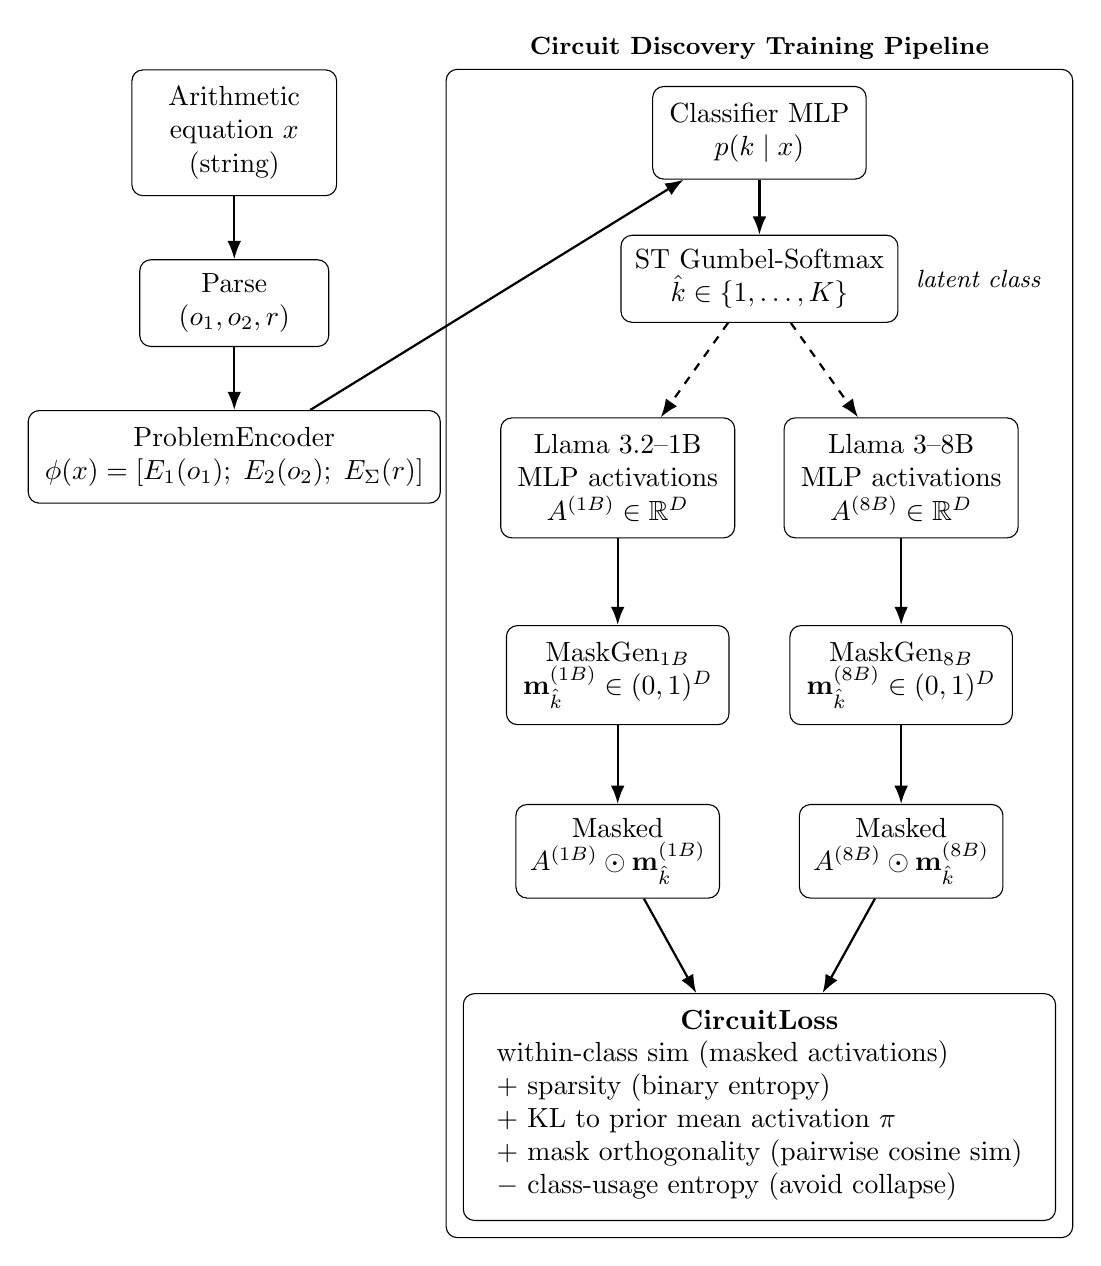
\begin{tikzpicture}[node distance=1.0cm and 1.5cm]
    
    \node[box] (eq) {Arithmetic\\equation $x$\\(string)};
    \node[sbox, below=0.8cm of eq] (parse) {Parse\\$(o_1,o_2,r)$};
    \node[box, below=0.8cm of parse] (enc) {ProblemEncoder\\
    $\phi(x)=[E_1(o_1);\;E_2(o_2);\;E_\Sigma(r)]$};
    
    \node[box, right=4.0cm of eq] (clf) {Classifier MLP\\$p(k\mid x)$};
    \node[sbox, below=0.7cm of clf] (gumbel) {ST Gumbel-Softmax\\$\hat{k}\in\{1,\dots,K\}$};
    \node[note, right=0.1cm of gumbel] {\emph{latent class}};
    
    \node[box, below=1.2cm of gumbel, xshift=-1.8cm] (acts1b) {Llama 3.2--1B\\MLP activations\\$A^{(1B)}\in\mathbb{R}^{D}$};
    \node[box, below=1.2cm of gumbel, xshift=1.8cm] (acts8b) {Llama 3--8B\\MLP activations\\$A^{(8B)}\in\mathbb{R}^{D}$};
    
    \node[box, below=1.1cm of acts1b] (mask1b) {MaskGen$_{1B}$\\
    $\mathbf{m}^{(1B)}_{\hat{k}}\in(0,1)^{D}$};
    \node[box, below=1.1cm of acts8b] (mask8b) {MaskGen$_{8B}$\\
    $\mathbf{m}^{(8B)}_{\hat{k}}\in(0,1)^{D}$};
    
    \node[sbox, below=1.0cm of mask1b] (masked1b) {Masked\\$A^{(1B)}\odot \mathbf{m}^{(1B)}_{\hat{k}}$};
    \node[sbox, below=1.0cm of mask8b] (masked8b) {Masked\\$A^{(8B)}\odot \mathbf{m}^{(8B)}_{\hat{k}}$};
    
    \node[box, below=1.2cm of masked1b, xshift=1.8cm, minimum width=5.5cm] (loss) {
    \textbf{CircuitLoss}\\[2pt]
    \begin{tabular}{l}
    within-class sim (masked activations)\\
    + sparsity (binary entropy)\\
    + KL to prior mean activation $\pi$\\
    + mask orthogonality (pairwise cosine sim)\\
    $-$ class-usage entropy (avoid collapse)
    \end{tabular}
    };
    
    \draw[line] (eq) -- (parse);
    \draw[line] (parse) -- (enc);
    \draw[line] (enc) -- (clf);
    \draw[line] (clf) -- (gumbel);
    
    \draw[dashedline] (gumbel) -- (acts1b);
    \draw[dashedline] (gumbel) -- (acts8b);
    
    \draw[line] (acts1b) -- (mask1b);
    \draw[line] (acts8b) -- (mask8b);
    
    \draw[line] (mask1b) -- (masked1b);
    \draw[line] (mask8b) -- (masked8b);
    
    \draw[line] (masked1b) -- (loss);
    \draw[line] (masked8b) -- (loss);
    
    \node[draw, rounded corners, inner sep=6pt, fit=(clf) (gumbel) (acts1b) (acts8b) (mask1b) (mask8b) (masked1b) (masked8b) (loss),
    label={[font=\small]above:\textbf{Circuit Discovery Training Pipeline}}] (fitbox) {};
    
    \end{tikzpicture}
    \caption{Circuit discovery architecture. Problems are embedded and assigned to a latent class via a straight-through Gumbel-Softmax classifier. The sampled class selects a class-conditioned neuron mask for each teacher model (1B and 8B), which gates flattened MLP activations. Training optimizes a multi-term objective encouraging within-class functional similarity, sparse masks, distinct circuits, and balanced class usage.}
    \label{fig:circuit-discovery-arch}
\end{figure}

\newpage
\section{Circuit Discovery Training Dynamics}
\label{app:training-dynamics}

\begin{figure}[H]
    \centering
    \includegraphics[width=0.92\linewidth]{figures/training_dynamics/cd_sparsify.png}
    \caption{Circuit discovery training curves related to sparsity regularization (binary-entropy sparsity loss and KL-to-prior mean activation). These curves support the discussion in Section~4.5.}
    \label{fig:cd-training-sparsity}
\end{figure}

\begin{figure}[H]
    \centering
    \includegraphics[width=0.92\linewidth]{figures/training_dynamics/cd_rep_ortho.png}
    \caption{Circuit discovery training curves related to representativeness (within-class similarity) and separation (mask orthogonality / cosine similarity). These curves support the discussion in Section~4.5.}
    \label{fig:cd-training-rep-ortho}
\end{figure}

\section{Circuit Distillation Training Dynamics}
\label{app:distillation_dynamics}

We visualize the training run for the Circuit Distilled student (Llama-3.2-1B). The model was trained for 50 epochs with $\lambda=0.01$.

\begin{figure}[H]
    \centering
    \begin{subfigure}[b]{0.49\textwidth}
        \centering
        \includegraphics[width=\linewidth]{figures/cka/accuracy.png}
        \caption{Student Test Accuracy}
        \label{fig:distill_acc}
    \end{subfigure}
    \hfill
    \begin{subfigure}[b]{0.49\textwidth}
        \centering
        \includegraphics[width=\linewidth]{figures/cka/ce_loss_steps.png}
        \caption{Cross Entropy Loss}
        \label{fig:distill_ce}
    \end{subfigure}
    
    \vspace{0.5cm}
    
    \begin{subfigure}[b]{0.49\textwidth}
        \centering
        \includegraphics[width=\linewidth]{figures/cka/cka_loss_steps.png}
        \caption{CKA Loss (Mechanism Alignment)}
        \label{fig:distill_cka}
    \end{subfigure}
    \hfill
    \begin{subfigure}[b]{0.49\textwidth}
        \centering
        \includegraphics[width=\linewidth]{figures/cka/loss_steps.png}
        \caption{Total Combined Loss}
        \label{fig:distill_total}
    \end{subfigure}
    
    \caption{Training dynamics for Circuit Distillation. The student rapidly acquires task accuracy (a) as the cross-entropy loss drops (b). Simultaneously, the CKA loss (c) steadily decreases, indicating that the student's internal representations in critical layers are becoming increasingly isomorphic to the teacher's layers.}
    \label{fig:full_dynamics}
\end{figure}

\newpage
\section{Hyperparameter Sensitivity and Failed Runs}
\label{app:failed_run}

To assess the robustness of our method, we report a failed training run where the representational alignment weight was increased to $\lambda=0.05$ and the learning rate to $2\times10^{-4}$.

\begin{figure}[H]
    \centering
    \begin{subfigure}[b]{0.49\textwidth}
        \centering
        \includegraphics[width=\linewidth]{figures/cka-old/accuracy.png}
        \caption{Student Test Accuracy (Failed Run)}
        \label{fig:fail_acc}
    \end{subfigure}
    \hfill
    \begin{subfigure}[b]{0.49\textwidth}
        \centering
        \includegraphics[width=\linewidth]{figures/cka-old/loss_steps.png}
        \caption{Total Loss (Failed Run)}
        \label{fig:fail_loss}
    \end{subfigure}
    
    \caption{Training dynamics for the failed run ($\lambda=0.05, \text{LR}=2\times10^{-4}$). The model fails to acquire the arithmetic capability, hovering near 0\% accuracy. The loss curves indicate optimization instability where the model likely collapsed or failed to escape a poor local minimum.}
    \label{fig:failed_dynamics}
\end{figure}

\textbf{Analysis of Failure:}
\begin{itemize}
    \item \textbf{Competing Objectives:} With a higher $\lambda=0.05$, the CKA loss dominates the gradient updates. This forces the student model to prioritize mimicking the teacher's exact high-dimensional topology over minimizing the token-prediction error (Cross Entropy). Since the student (1B) has significantly less capacity than the teacher (8B), satisfying the strict geometric constraints of the teacher's representation may be incompatible with the student's own optimal path to the solution.
    \item \textbf{Optimization Instability:} The higher learning rate ($2\times10^{-4}$) likely exacerbated this conflict, causing the optimizer to oscillate rather than converge. This suggests that mechanism-level distillation requires a delicate balance: the alignment signal must be strong enough to guide the student towards the correct circuit, but weak enough to allow the student to adapt that circuit to its own compressed latent space.
\end{itemize}

\newpage
\section{Supervised Circuit Distillation (Beating the Teacher)}
\label{app:supervised_distillation}

We explored a variation of our method where we replaced the standard distillation loss (matching student logits to teacher logits) with a standard Cross-Entropy loss against the \textbf{ground truth labels}, while maintaining the mechanism alignment ($\lambda=0.01$ CKA).

\begin{figure}[H]
    \centering
    \begin{subfigure}[b]{0.49\textwidth}
        \centering
        \includegraphics[width=\linewidth]{figures/cka-loss/accuracy.png}
        \caption{Student Accuracy (Ground Truth Supervision)}
        \label{fig:sup_acc}
    \end{subfigure}
    \hfill
    \begin{subfigure}[b]{0.49\textwidth}
        \centering
        \includegraphics[width=\linewidth]{figures/cka-loss/loss_steps.png}
        \caption{Total Loss}
        \label{fig:sup_loss}
    \end{subfigure}
    
    \caption{Training dynamics when distilling circuits using Ground Truth labels. The student not only converges but eventually surpasses the teacher's baseline accuracy of 96.3\%, achieving near-perfect performance. This indicates that the 1B model has sufficient capacity to solve the task perfectly when guided by correct mechanisms.}
    \label{fig:supervised_dynamics}
\end{figure}
Standard knowledge distillation is often limited by the teacher's own performance (96.3\% in our baseline). By using hard ground-truth labels, the student is not penalized for "correcting" the teacher's mistakes.
\end{document}
